\chapter{The Large Hadron Collider and the CMS experiment}

This work is based on data collected by the Compact Muon Solenoid (CMS) experiment, 
one of the four main experiments together studying the collisions 
provided by the Large Hadron Collider (LHC). A detailed description of the LHC and of the CMS 
experiment can be found in \cite{Evans:2006tq} and \cite{Chatrchyan:2008aa} respectively.
In this chapter we summarize the main features that are relevant for this work.

\section{The Large Hadron Collider}

The LHC and its experiments were built to explore the high-energy frontier of particle physics and to address fundamental questions of this field such as the existance of a Higgs boson \cite{Englert:1964et,Higgs:1964ia,Higgs:1964pj,Guralnik:1964eu,Higgs:1966ev,Kibble:1967sv}, of extended symmetries \cite{Martin:1997ns}, extra dimensions \cite{Antoniadis:1999bq} or new elementary particles \cite{Beltran:2010ww,Randall:1999vf}. All these phenomena don't have a well-defined energy range predicted by theory even though are expected to manifest at the TeV scale. A proton-proton collider was considered to be the most suitable machine for such a task, allowing higher energies with current technologies and probing wider energy ranges at the same time exploiting the compositeness of the colliding particles.

The LHC is housed in the 27 km long underground tunnel where the Large Electron Positron collider (LEP) has been operating until its decommissioning in 2000. The tunnel is located under both French and Swiss territory, in proximity of the CERN research facility. Before being accelerated in the LHC protons are produced from hydrogen ionization and then accelerated through a chain of smaller machines, some of them dating back to the late 1950's. A schematic view of the CERN accelerators and their connection is shown in Figure \ref{fig:cern_accelerators}. From the last element of this chain, the Super Proton Syncrotron (SPS), protons are injected in the LHC with an energy of 450 GeV in two separate beam pipes, one containing protons running clockwise, the other with protons running in the opposite direction. Protons are bent in their trajectory by 1\,232 superconducting dipole magnets and focused by  superconducting quadrupole magnets, while 16 superconducting radio-frequency (RF) stations 
%provide the thrust to 
accelerate the two beams up to 7 TeV in steps of 0.5 MeV each turn. In order to maintain superconducting properties the magnet coils and the cavities are cooled to 1.9 K by a complex cryogenic system using superfluid helium as refrigerator. RF cavities can be used for accelerating the protons only if the beam is not continuous but structured in bunches. By design the LHC is built to contain 2808 bunches of $10^{11}$ protons each, giving a bunch time separation of 25 ns.
%Due to space constraints both the beam pipes are encased in the same dipole and the proper magnetic field direction is achieved with a particular magnet design.  

\begin{figure}
\begin{center}
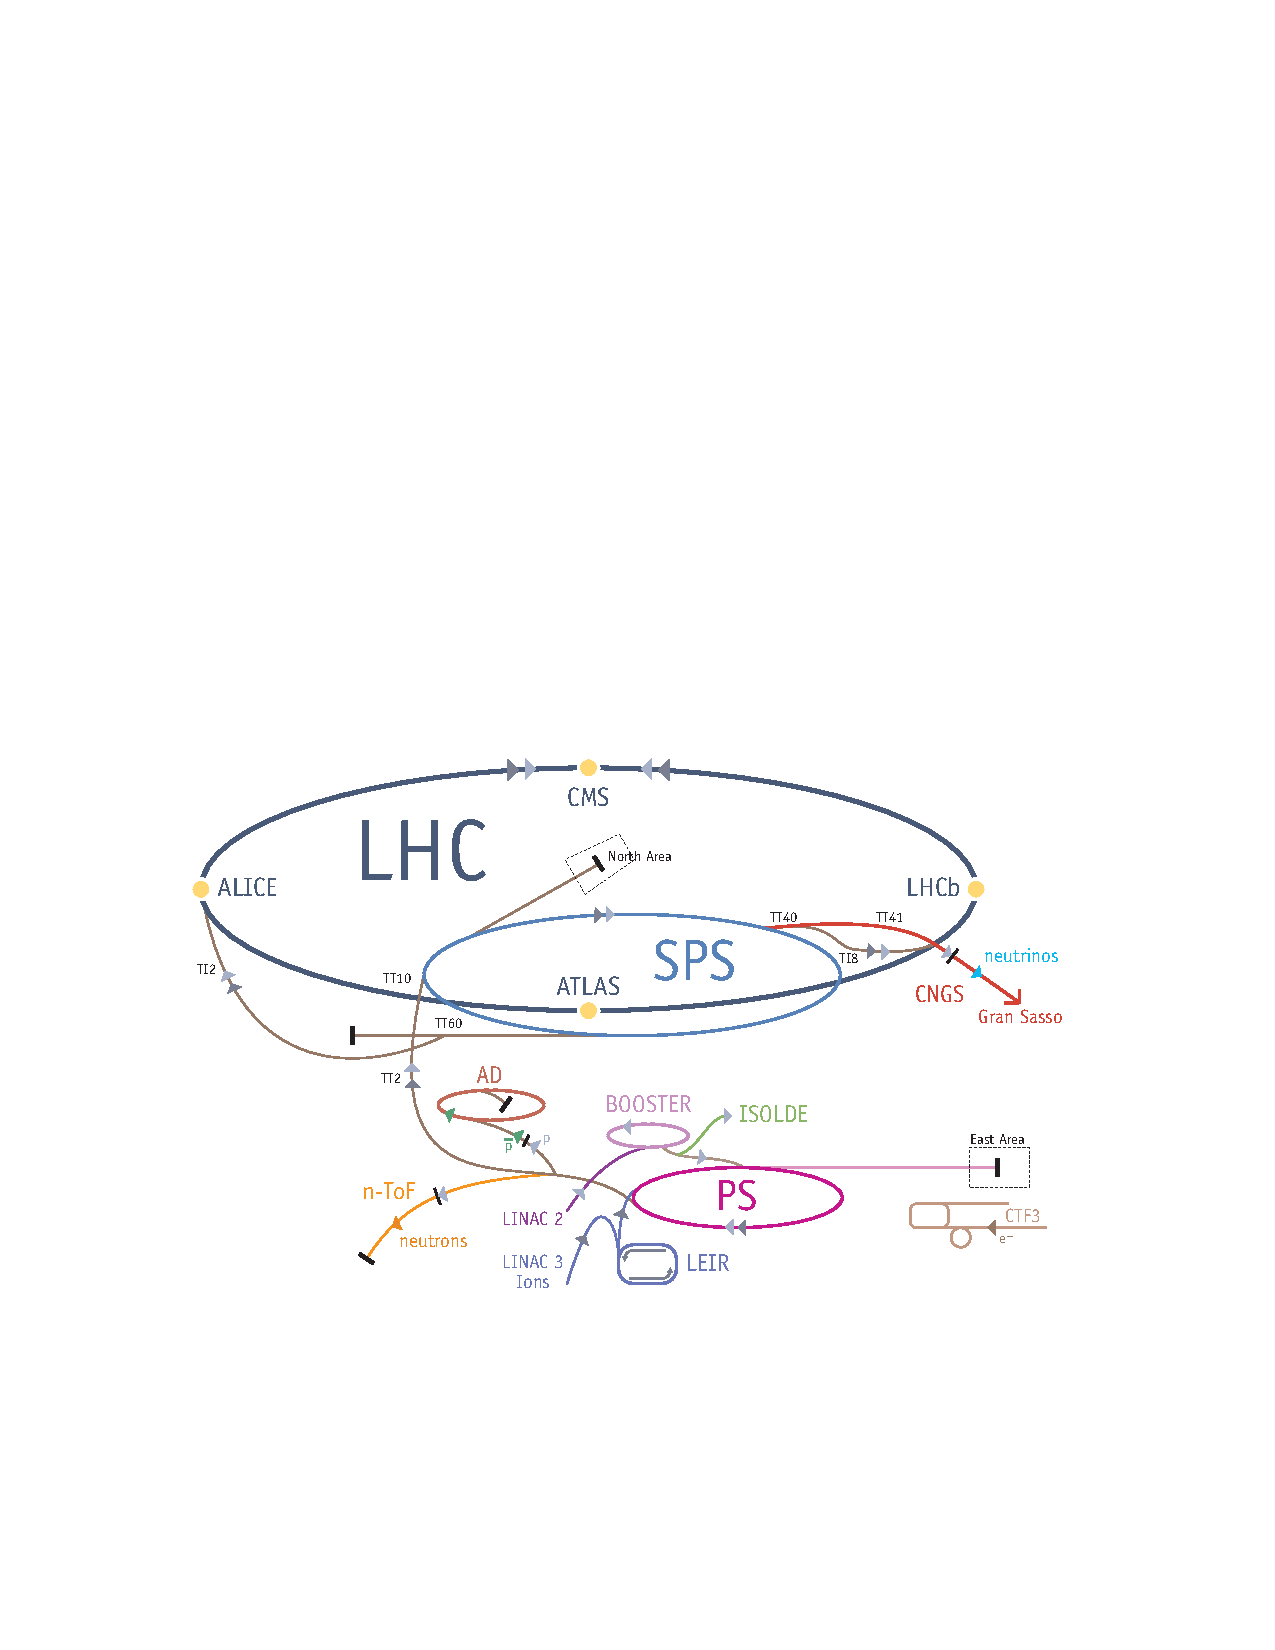
\includegraphics[angle=-0,width=0.8\textwidth]{2_LHC_and_CMS/pics/LHC.pdf}
\caption{Schematic view of the CERN accelerators and their connection
\label{fig:cern_accelerators}
}
\end{center}
\end{figure}

The LHC started its operation on 10 September 2008 and after only 9 days of operation a severe \emph{quenching} of about 100 dipole magnets, causing the release of around two tones of helium, forced the machine to stop and to address some design figures. The main cause of the accident was found to be in some of the electrical connections between magnets. In 2009 the machine became again operational with a reduced beam energy, allowing for less current to flow in the dipole magnets. The year 2010, after a careful ramp-up of the beam energies, saw the start of the LHC research program with collisions at a center-of-mass energy $\sqrt{s} = 7$ TeV, half of the designed one. During 2010 and 2011 the machine commissioning continued along with data taking improving the instantaneous luminosity and allowing for an increase of the beam energy to 4 TeV that took place in 2012. The LHC design specifications and achieved ones are summarized in table \ref{tab:lhc_figures}.

\begin{table}[h!]
   \centering
\begin{tabular}{c|ccccc}
\hline
Parameter & Design value&  Best value achieved \\ 
\hline
Beam energy   & 7 TeV & 4 TeV \\ 
Number of protons per bunch & 1.15$\times$10$^{11}$ & 1.5$\times$10$^{11}$ \\
Number of bunches & 2808 & 1368 \\
Crossing angle & 300~\si{\micro\metre} & 290~\si{\micro\metre} \\
Beam size & 17~\si{\micro\metre} & 20~\si{\micro\metre} \\
Emittance & 3.75 ~\si{\micro\metre} & 2.4~\si{\micro\metre}  \\
Peak luminosity & $10^{34}$~cm$^{-2}$s$^{-1}$ & 7.5$\times$10$^{33}$~cm$^{-2}$s$^{-1}$ \\
\hline
\end{tabular}
  \caption{Relevant LHC machine parameters. The design values are compared to the ones reached during the 2013 operations.}
  \label{tab:lhc_figures}                
\end{table}


The instantaneous luminosity,$\operatorname{\mathcal{L}}(t)$, is the number of particles per unit area per unit time available for collisions. For any given physics process the average number events is given by:

\begin{equation} 
	N_{ev} = \sigma\int\operatorname{\mathcal{L}}(t)\mathrm{d}t
	\label{eq:n_events}
\end{equation} 

where $\sigma$ is the cross-section for such process. While the cross section depends on the scattering process, the instantaneous luminosity can be entirely derived from accelerator figures:

\begin{equation} 
	\operatorname{{\cal L}}(t) = \frac{N_p^2 n_b f_{rev} \gamma }{4 \pi \epsilon_{n} \beta^*} F
	\label{eq:lumi}
\end{equation} 

where $N_p$ and $n_b$ are the number of protons per bunch and the total number of bunches respectively, $f_{rev}$ is the rotation frequency, $\epsilon_{n}$ and $\beta^*$ describe the beam focusing at the interaction point, $\gamma$ is a relativistic factor and $F$ accounts for the crossing angle between the two beams. Although the number of bunches has always been less than half the design value during all the running period, the peak instantaneous luminosity has only been 30\% lower than the design one. This result was achieved by increasing the number of protons in each bunch and increasing the focusing of the beams, at the price of increasing the average number of proton collisions per bunch crossing, the so-called \emph{pileup}. This effect is displayed in figure \ref{fig:lhc_pileup} where the peak number of simultaneous interactions per bunch crossing recorded by the CMS detector shown as a function of time.

\begin{figure}
\begin{center}
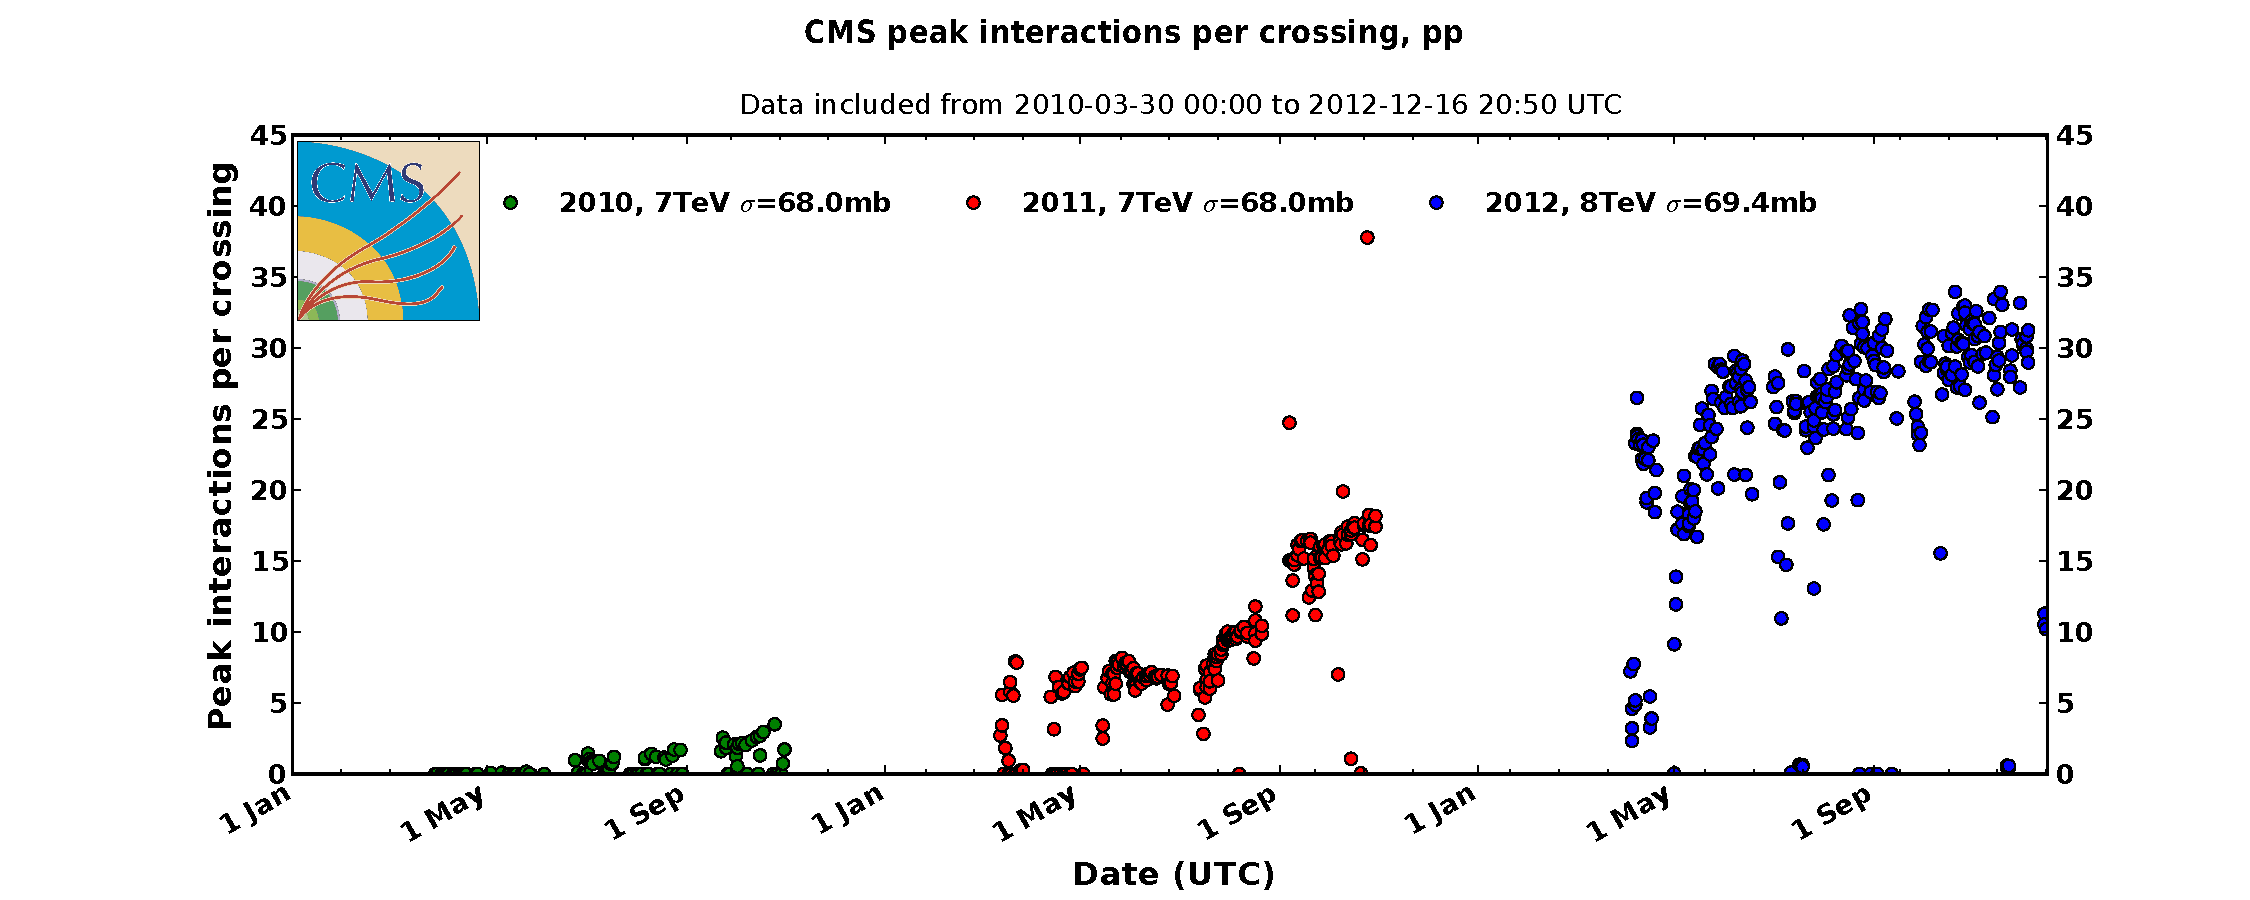
\includegraphics[angle=-0,width=\textwidth]{2_LHC_and_CMS/pics/peak_pu_pp.pdf}
\caption{Peak number of interactions per bunch crossing in function of time as recorded by the CMS detector
\label{fig:lhc_pileup}
}
\end{center}
\end{figure}

As can be clearly seen by Eq. \ref{eq:n_events}, the most important figure for physics searches is the integrated luminosity which is usually quoted as \L. During its operations LHC delivered 44.2~pb\Inv in 2010, 6.1~fb\Inv in 2011 and 23.3~fb\Inv at 8~TeV in 2012. The huge progress made by the accelerator in terms of integrated luminosity can be clearly seen in figure \ref{fig:int_lumi}.

\begin{figure}
\begin{center}
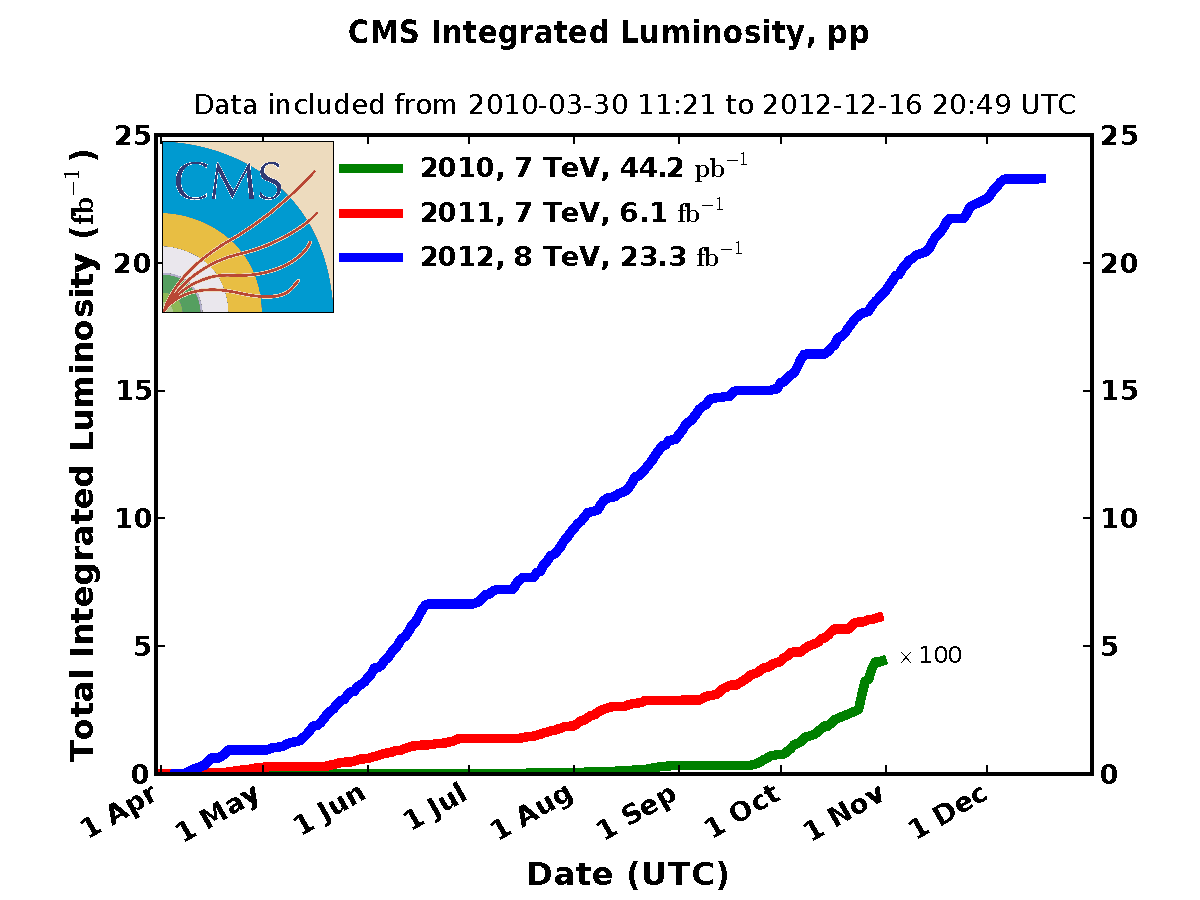
\includegraphics[angle=-0,width=0.8\textwidth]{2_LHC_and_CMS/pics/int_lumi.pdf}
\caption{Cumulative luminosity versus day delivered to CMS during stable beams and for p-p collisions. This is shown for 2010 (green), 2011 (red) and 2012 (blue) data-taking.
\label{fig:int_lumi}
}
\end{center}
\end{figure}


\section{The CMS detector}

The CMS detector is located in the LHC tunnel at point 5, near the French town of Cessy, between the Jura mountains and the Geneva lake.
 
The CMS experiment, together with ATLAS, is one of the two multi-purpose detectors operating at the LHC. Its primary task is to probe particle physics at the TeV scale looking for new phenomena and for the Higgs boson, the only missing piece to the SM puzzle. The experiment is also well suited to perform precision measurements of standard model processes and flavor physics studies. A heavy-ion program is carried on as well to probe QCD at very high energies and matter densities, trying to reproduce an environment similar to the conditions of the universe few instants after the Big Bang.

To carry out such ambitious research program the detector was designed to meet some baseline requirements:
\begin{itemize}
\item Good muon identification and momentum resolution over a wide range of momenta and angles with di-muon mass resolution of ~1\% at 100~GeV.
\item Ability to identify the muon charge without any ambiguity for muons momenta below 1~TeV
\item Good charged-particle momentum resolution, high tracking efficiency and resolution. This two figures are especially important for objects like \b-jets and tau leptons, where isolated charged hadrons and displaced vertices play a fundamental role. A high tracking resolution also plays a key role in assigning the tracks to the production vertex mitigating the effect of pileup.
\item Good electromagnetic energy resolution, with a di-photon invariant mass resolution of \~1\% at 100~GeV and wide geometric coverage with efficient photon and lepton isolation in high pileup conditions.
\item Hermetic hadronic calorimeter with fine transverse segmentation for good jet mass and missing transverse energy ($E_T^{miss}$) resolution. 
\end{itemize}

The total proton-proton cross section at 14~TeV is expected to be roughly 100~mb, with LHC design values it is therefore expected an average of 20 inelastic collisions for each bunch crossing, a value that was widely overcome during the 2012 run. The number of overlapping events (\emph{pileup}) together with the short 25~ns bunch spacing pose stringent requirements on the resolution, granularity and latency of the different subdetectors. The ability to resolve overlapping vertices and assign their respective track is of primary importance. A fast trigger system is also required to reduce the event rate from the collision rate of 40~MHz to 300Hz which can be permanently stored.

In order to meet all these requirements CMS has been built with a 4~T NbTi superconducting solenoid magnet with an inner diameter of 6 m. Inside the magnet a large silicon tracker, the largest of its kind, is housed to track charged particles with the required resolution. Around the tracker, but still within the solenoid field a lead-tungstanate electromagnetic calorimeter (ECAL) and a brass-scintillating sampling hadron calorimeter (HCAL). Inside the 1.5~m thick iron return yoke of the magnet four muon stations are installed. They consist of several layers of drift tubes or cathode strip chambers complemented by resistive plate chambers. A schematic view of a transverse CMS slice is presented in figure \ref{fig:cmsdet}

\begin{figure}
\begin{center}
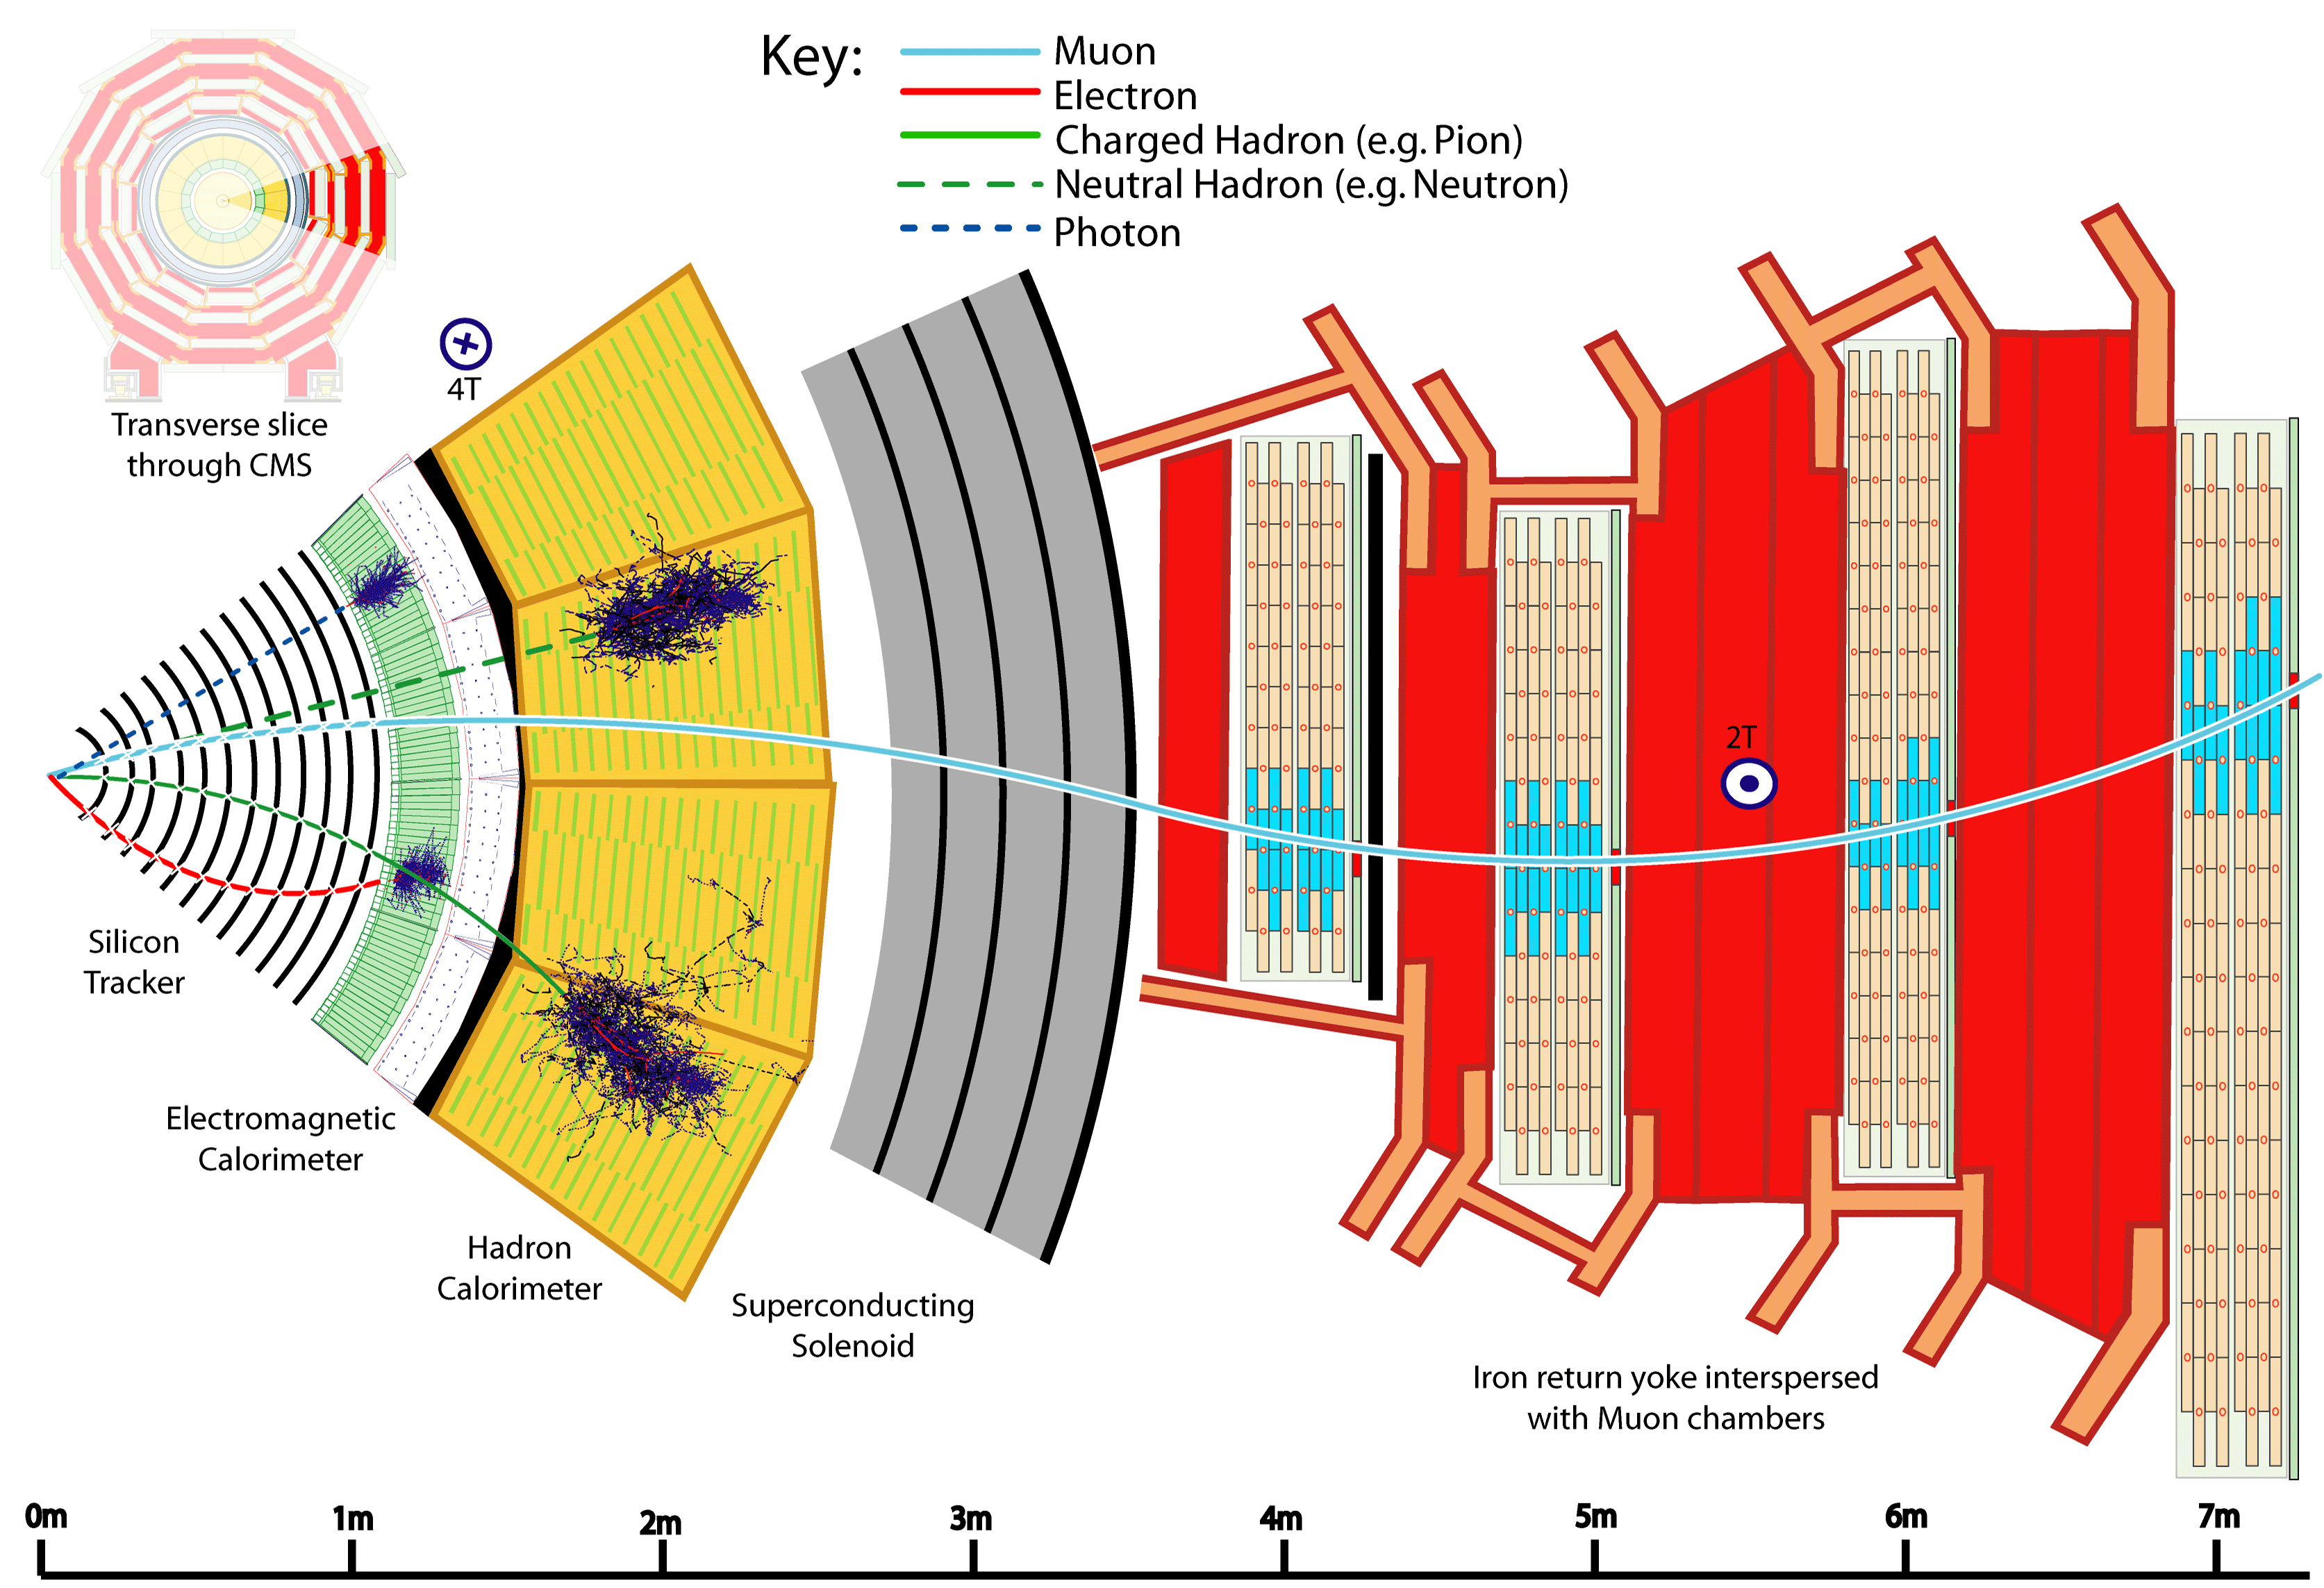
\includegraphics[angle=-0,width=0.8\textwidth]{2_LHC_and_CMS/pics/CMS_Slice_HD.png}
\caption{transverse slice of the CMS barrel section showing the trajectory for different particles with and the signal deposed in each subdetector.
\label{fig:cmsdet}
}
\end{center}
\end{figure}


\paragraph{The coordinate system}
chosen for CMS sets the $y$ axis vertical pointing upwards and the $x$ axis horizontal pointing towards the center of LHC, therefore the $z$ axis is placed along the beam line pointing in the direction of the beam running anti-clockwise or towards the Jura. An additional set of polar coordinates is used to describe the $xy$ plane in the form of radius $r$ and angle $\phi$, while the angle $\theta$ is measured with respect to the positive $z$ axis direction. Usually the polar angle $\theta$ is replaced by the \emph{pseudorapidity}, defined as $\eta=-\ln \tan(\theta/2)$, is Lorentz invariant for boosts along the $z$ axis and therefore comes very handy when describing processes whose longitudinal boost is unknown. The three-dimensional angular distance is also replaced by its Lorentz-invariant $\D R=\sqrt{\D\phi^2+\D\eta^2}$, where $\D\eta$ and $\D\phi$ are the $\eta$ and $\phi$ coordinate differences of two points.

\subsection{Inner Tracker}
\label{sec:inner_tracker}

The inner tracker provides the essential spatial informations needed to reconstruct charged tracks as well as primary and secondary vertices. A schematic view of the inner tracker is shown in figure \ref{fig:tracker}. To cope with the very high occupancy and to provide the best possible spatial resolution the innermost part of the tracker is based on silicon pixel technology. The pixel detector, displayed in figure \ref{fig:pixel}, is composed of three cylindrical layers at radii of 4.4, 7.3 and 10.2 cm complemented by four disks  in the forward/backward region. The total active area of the pixel detector is roughly of 1 m\sq~and its angular acceptance covers $|\eta| \leq 2.5$, providing three bi-dimensional measurements over the full acceptance. The pixel cell size is 100 $\times$ 150 \u m\sq. The ionization charge is shared between neighboring pixels due to the solenoidal magnetic field. To enhance this effect in the forward wheels the sensors are placed in a turbine shape. The analogue read-out and charge sharing allow for a 9-33 \u m resolution \cite{trackingpaper}. 

The pixel detector can be extracted from the rest of the tracker to allow easy access for maintenance without interfering with the rest of the detector. This feature is particularly important due to the high radiation dose that the first layers of the pixel detector sustain, requiring additional maintenance.

\begin{figure}
\begin{center}
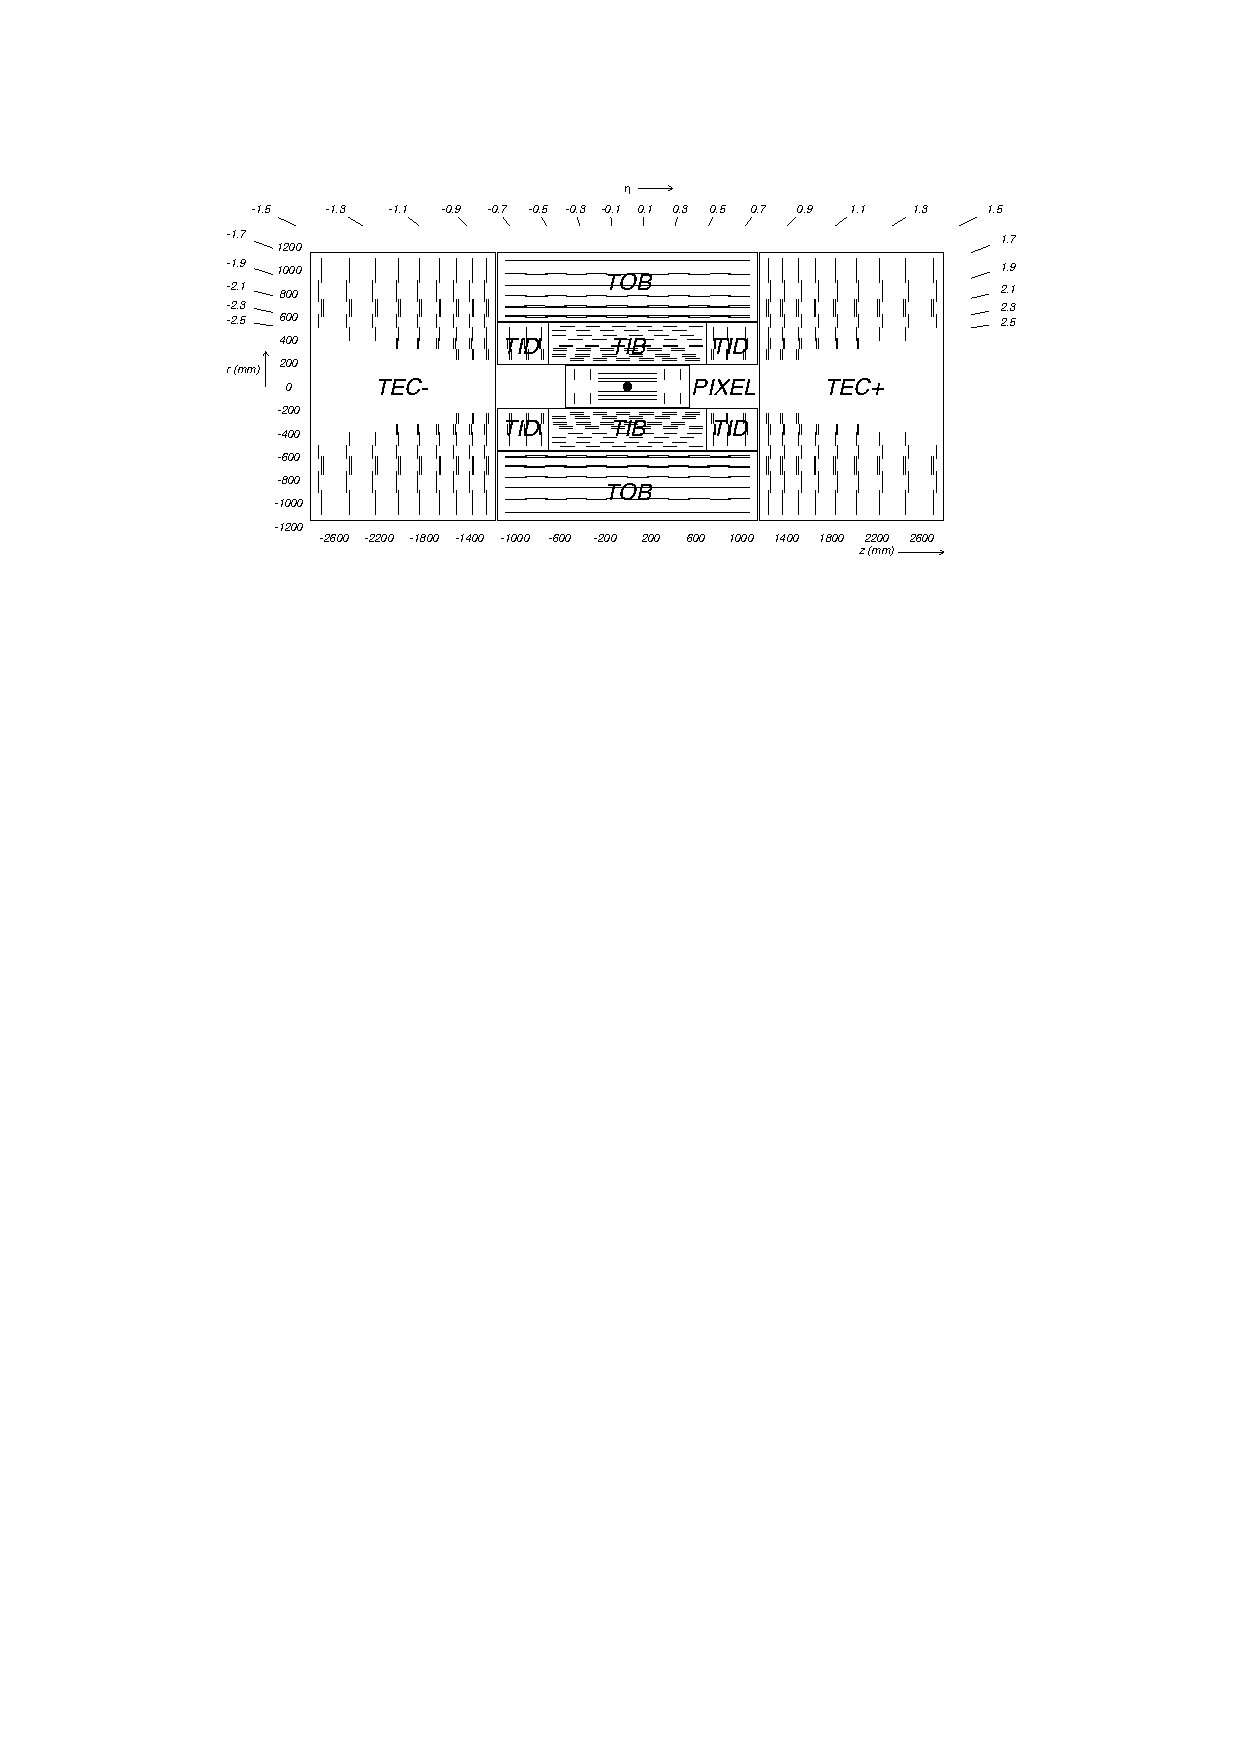
\includegraphics[angle=-0,width=0.8\textwidth]{2_LHC_and_CMS/pics/trkxsec.pdf}
\caption{Longitunal cross section of the CMS tracker with pseudo rapidity coverage. 
\label{fig:tracker}
}
\end{center}
\end{figure}

\begin{figure}
\begin{center}
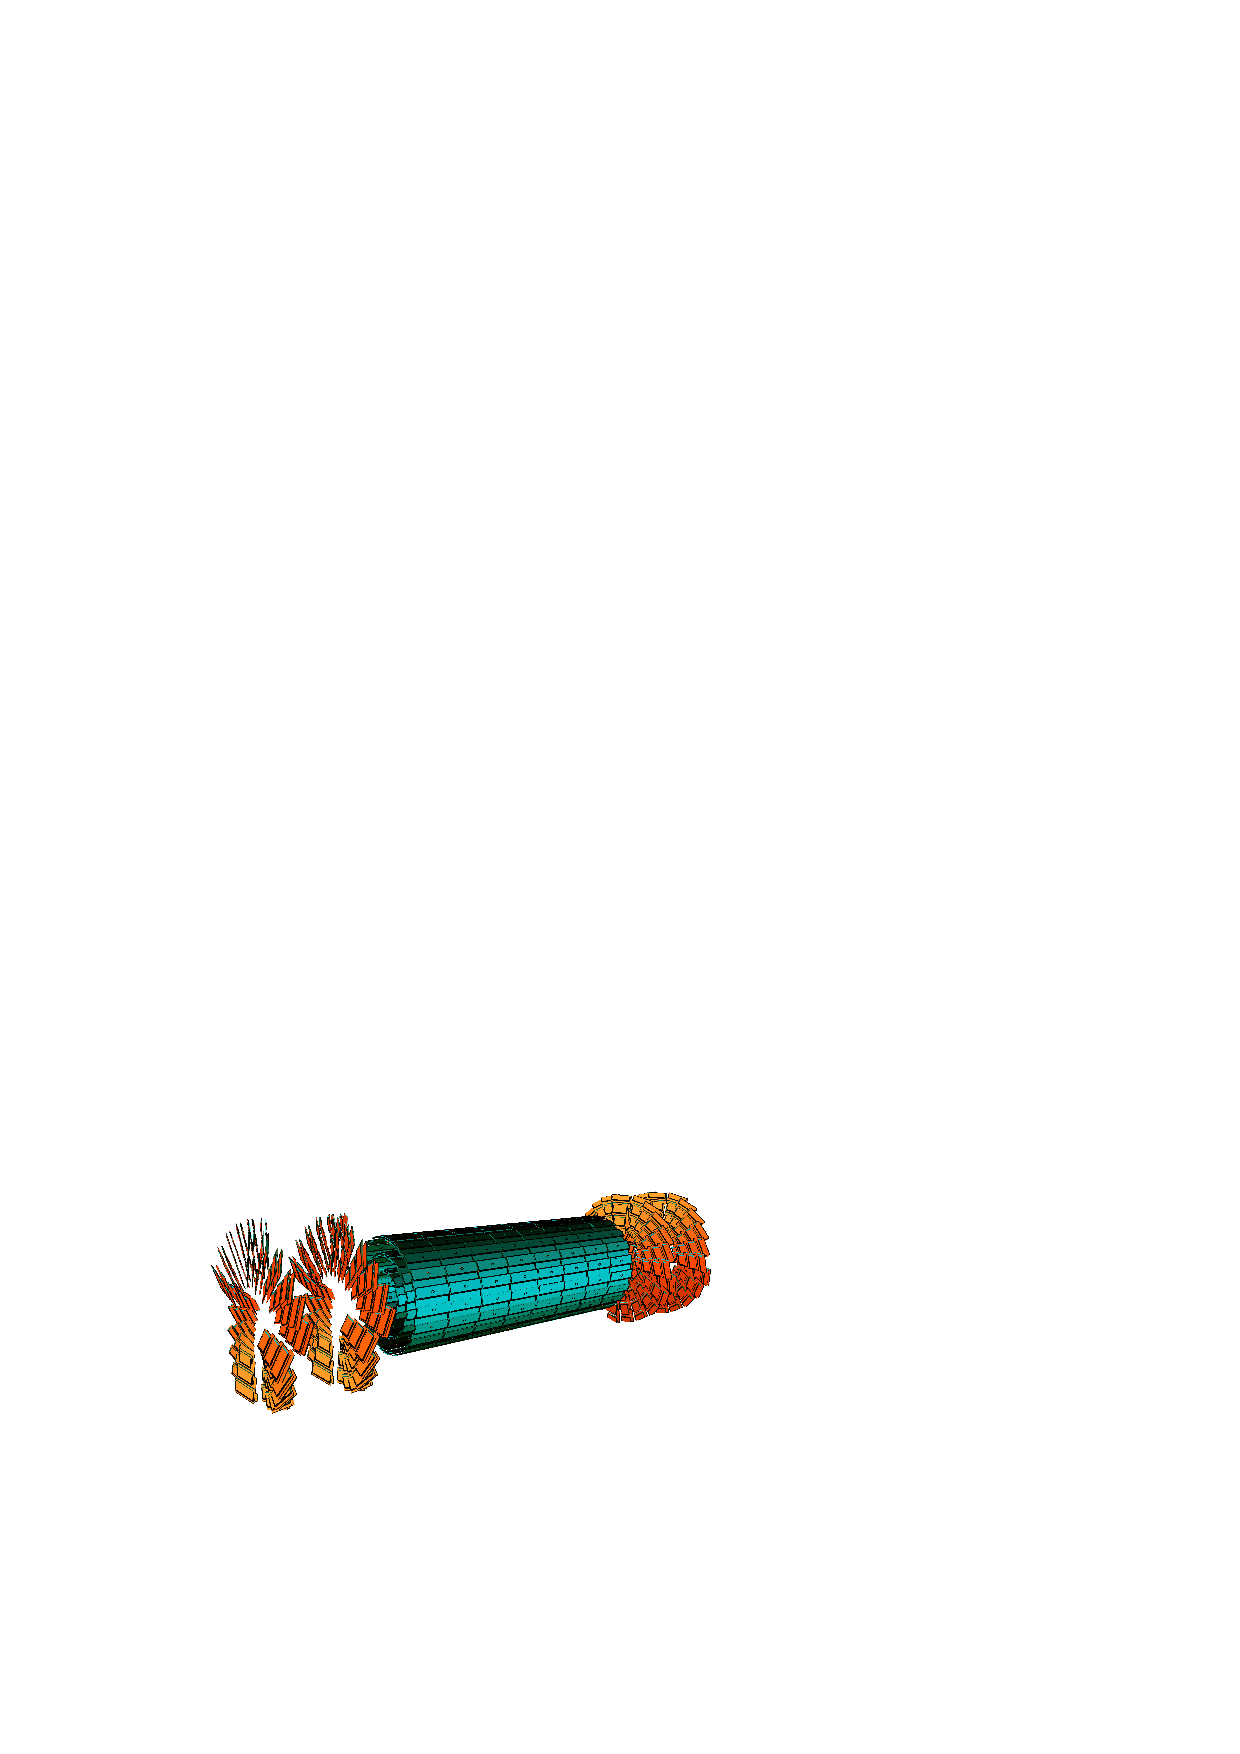
\includegraphics[angle=-0,width=0.8\textwidth]{2_LHC_and_CMS/pics/pixelfull.pdf}
\caption{Three dimensional sketch of the CMS pixel detector, barrel modules in blue and endcap wheels in orange.
\label{fig:pixel}
}
\end{center}
\end{figure}

The outer layers of the tracker are made of silicon strip detectors and further divided into four sections: Tracker inner and outer barrel (TIB and TOB), tracker inner disks (TID) and tracker endcaps (TEC). TIB and TID are located at radii between 20 and 55 cm from the beam line. They consists of four barrel layers and three disks at each end. The sensors are made of 320 \u m thick silicon with a strip pitch that varies from 80 \u m in the innermost barrel layer to 140 \u m in the outermost disks. The combination of TIB and TID delivers up to four transverse measurements. The TIB-TID sections are surrounded by the TOB, which fills the remaining space up to a radius of 116 from the beam line. It consists of six barrel layers of 500 \u m thick sensors with a strip pitch of 183 \u m for the first four layers and 122 \u m for the remaining two. The TEC is located in the end-cap region, for radii larger than 20 cm and $|z| > 118$ cm. The TEC consist in nine disks composed by up to seven concentric rings of strip sensors. The thickness and the strip pitch of the sensor varies depending on the distance of the ring from the beam line. 

Intrinsically strip sensors only provide one dimensional measurement ($\phi$), to achieve the measurement of the second coordinate ($r$ for disks, $z$ for barrel) an additional set of sensors is mounted back-to-back with a stereo angle of 100 mrad on the first two layers of TIB, TID and TOB and on layers 1, 2 and 5 of TEC. This layout ensures about 9 hits in the strip tracker acceptance with at least four of them being two-dimensional.

%temperatura?

\subsection{Electromagnetic Calorimeter}

The CMS electromagnetic calorimeter (ECAL) is located around the inner tracker. It is divided into ECAL Barrel (EB) covering the pseudo rapidity range of $|\eta| < 1.479$ and ECAL Endcaps (EE) which cover $1.479 < |\eta| < 3$. 
The calorimeter consist of 68\,524 scintillating lead tungstanate (PbWO$_4$) crystals readout by photomultipliers. 

The choice of lead tungstanate was driven by its high density yielding a short radiation length (0.89 cm) and small Moliere radius (2.2 cm) together with the radiation hardness and fast response, with 80\% of the light yield emitted within 25~ns. To keep the calorimeter as hermetic as possible the crystals have truncated pyramidal shape with one of the longitudinal faces left unpolished to moderate the non uniform light collection across the crystal length that this peculiar shape causes. Each crystal covers about $0.0174 \times 0.0174$ in $\eta-\phi$ plane and is oriented pointing towards the nominal interaction point with a slight misalignment to mitigate the effect of the crystal surface on photon detection. Each crystal is read-out by either a pair of avalanche photodiodes (APD) in the barrel or by vacuum phototriodes in the endcap. Both the devices can operate in high magnetic fields with little or no efficiency degradation. 

A pre-shower detector is installed in front of the ECAL endcap, with the purpose of discriminating between real photons and in-flight \piz decays and to enhance the angular resolution of both electrons and photons. The pre-shower detector consists of a double-layer lead-silicon calorimeter, with the lead initiating the shower and the silicon strip detector placed after each radiator measuring the deposited energy and shower profile with high granularity.

\subsection{Hadronic Calorimeter}

The hadronic calorimeter (HCAL) serves two purposes: it measures the energy of charged and neutral hadrons from the p-p interaction while stopping them, thus allowing only muons to pass through and avoiding large quantities of energy being deposited inside the superconducting magnet. As most of the other subdetectors HCAL is divided in a barrel section (HB), covering the acceptance region with $|\eta| < 1.3$, and an endcap section (HE) covering $1.3 < |\eta| < 3$. Both parts are located inside the superconducting solenoid. HCAL is a sampling calorimeter with brass passive plates, in which the hadronic shower begins and develops, interspaced with active plastic scintillator measuring  the shower development. 

The scintillator is segmented both in $\eta$ and in $\phi$ to provide the required granularity. Each scintillating tile is connected to the readout by a wavelength-shifting fiber that runs in a groove machined in the tile itself. Such fiber is thermally spliced to a clear fiber carrying the emitted light to a hybrid photodiode (HPD). HPD's consist of a photocathode kept at high voltage. Electrons emitted by the photocathode are accelerated in the short distance (\~3 mm) that separates the cathode from a silicon pixelated anode which amplifies the signal. These devices were chosen due to their high dynamic range, their high gain ($O(2000)$) and the possibility to work in a magnetic field.

The effective thickness of the calorimeter in terms of interaction length, $\lambda_I$, spans in the barrel from a minimum of 5.82 $\lambda_I$ at $\eta=0$ to a maximum of 10.6 $\lambda_I$ at $|\eta| = 1.3$. The ECAL crystals add about 1.1 additional interaction lengths. The total thickness of the endcap calorimeters, including in the ECAL crystals, is about 10 $\lambda_I$.

Due to the limited stopping power of HB, especially in the central rapidity region, an additional hadronic calorimeter is placed outside the solenoid magnet (hadron outer or HO) with the function of \emph{tail catcher}. HO consist of one scintillating station (two for the most central region) exploiting the solenoid itself ( and the first return yoke in case of the second station) as absorber. This additional detector extends the total thickness of the HB up to a minimum of $11 \lambda_I$.

\subsection{Muon System}

Muon detection and trigger is of prime importance as of many new physics processes may become manifest through decay chains involving muons. Among those the decay of a Higgs boson into $\Z\Z^*\To4\mu$ stands out as one of CMS's flagship analyses and one of those leading to the discovery of the Higgs boson announced on July 4$^{th}$, 2012 \cite{Chatrchyan:2013lba}. For this reason a redundant system of three different kinds of detectors is used to track muons in CMS. 

The muon system, whose scheme is shown in figure \ref{fig:mudet}, is housed in gaps between the return yoke of the solenoid magnet in the outermost region of the experiment. It consists of a Drift Tube (DT) tracking system in the barrel and multi-wire proportional chambers in the end-cap. In addition, a set of Resistive Plate Chambers (RPC) is located both in the barrel and in the endcap regions, providing a better time resolution  at the cost of coarser spatial resolution. 

\begin{figure}
\begin{center}
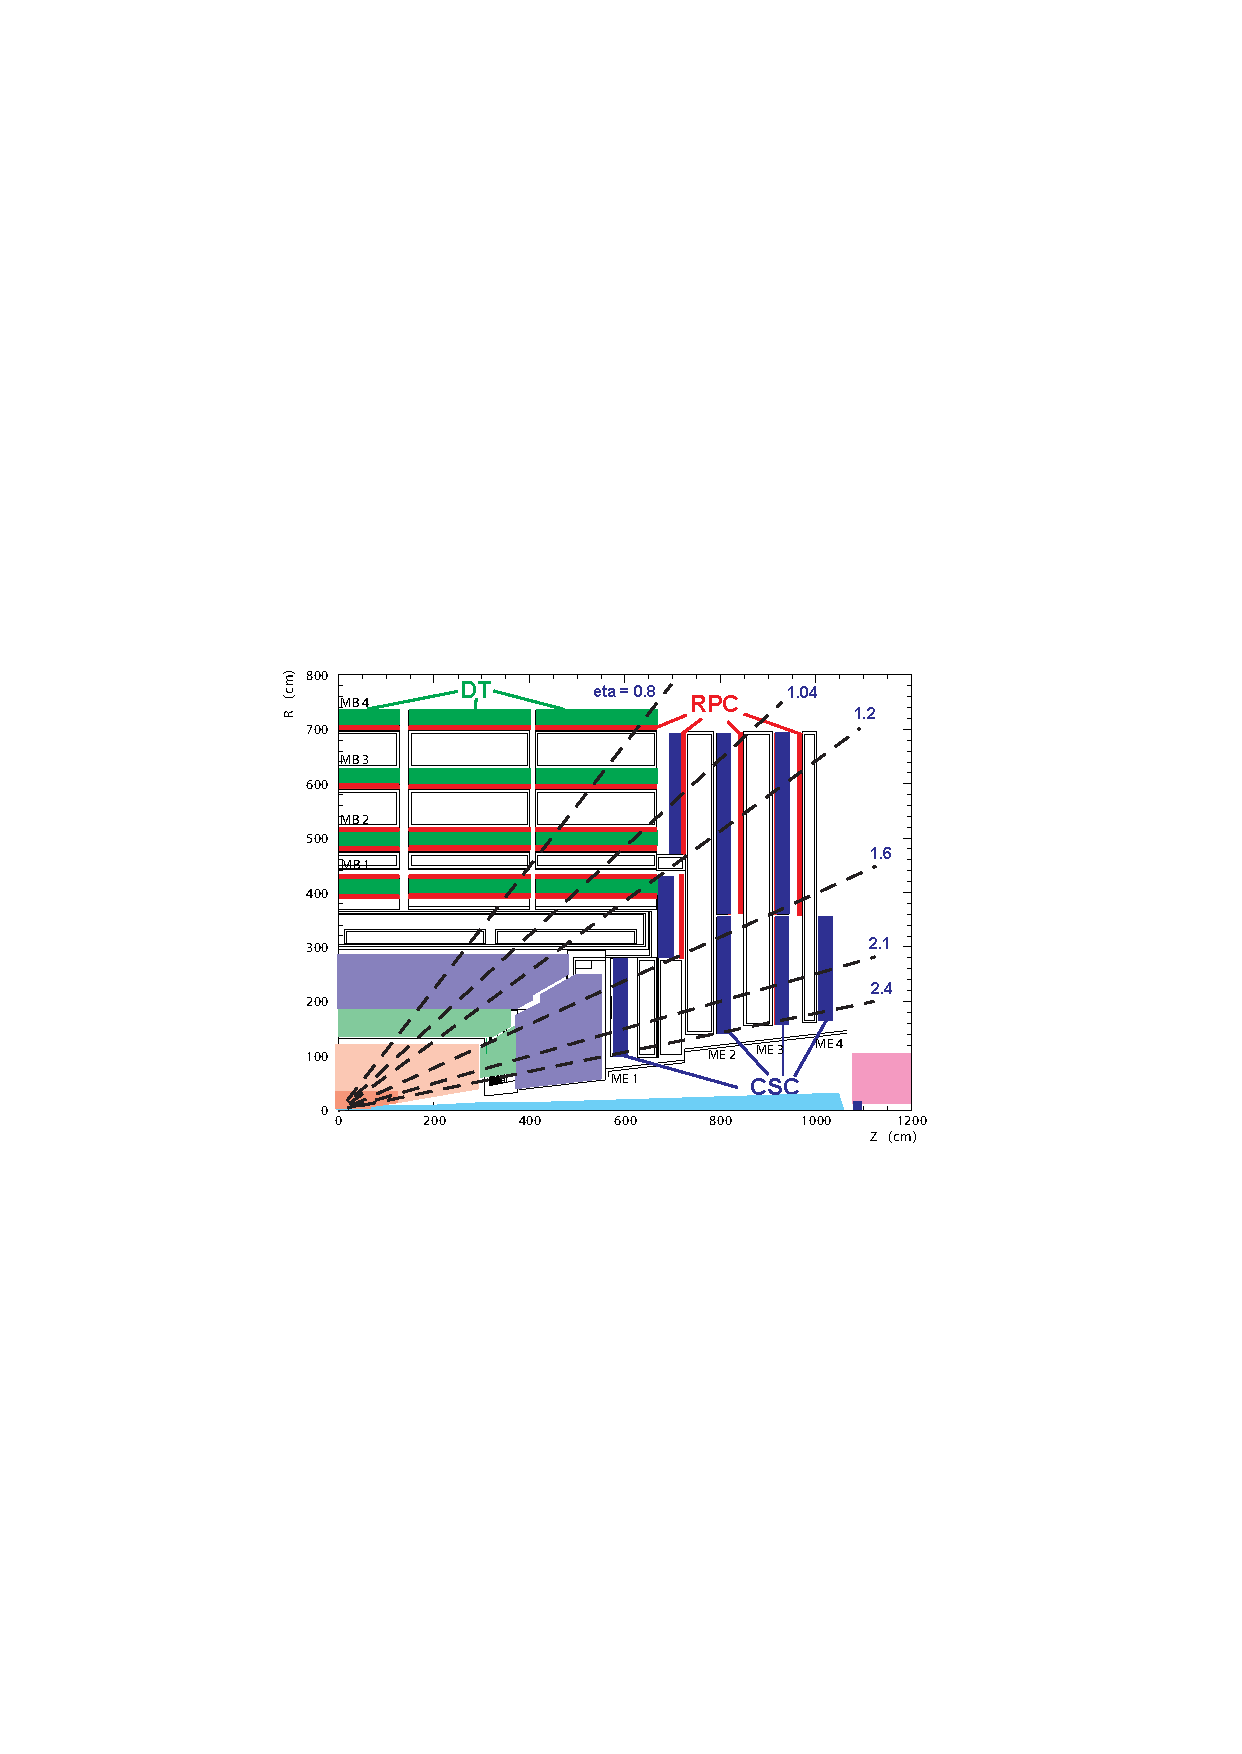
\includegraphics[angle=-0,width=0.8\textwidth]{2_LHC_and_CMS/pics/mudet.pdf}
\caption{Longitudinal cross-section of the CMS detector showing the location of the muon system.
\label{fig:mudet}
}
\end{center}
\end{figure}

\subsubsection*{Drift Tubes}

Drift tubes identify and track muons in the barrel region ($|\eta| < 1.2$) where the rate is below 1 Hz/cm\sq ~and residual magnetic field less than 1 T allowing the usage of this technology. Four station are located at increasing distance from the beam line. The first three stations are equipped with two \emph{super-layers} (SL) providing a measurement of $\phi$ and one SL measuring the $z$ coordinate, as can be seen in figure \ref{fig:dt_module}, representing one DT module. In the last two stations the SL measuring the $z$ coordinate is missing. 

\begin{figure}
\begin{center}
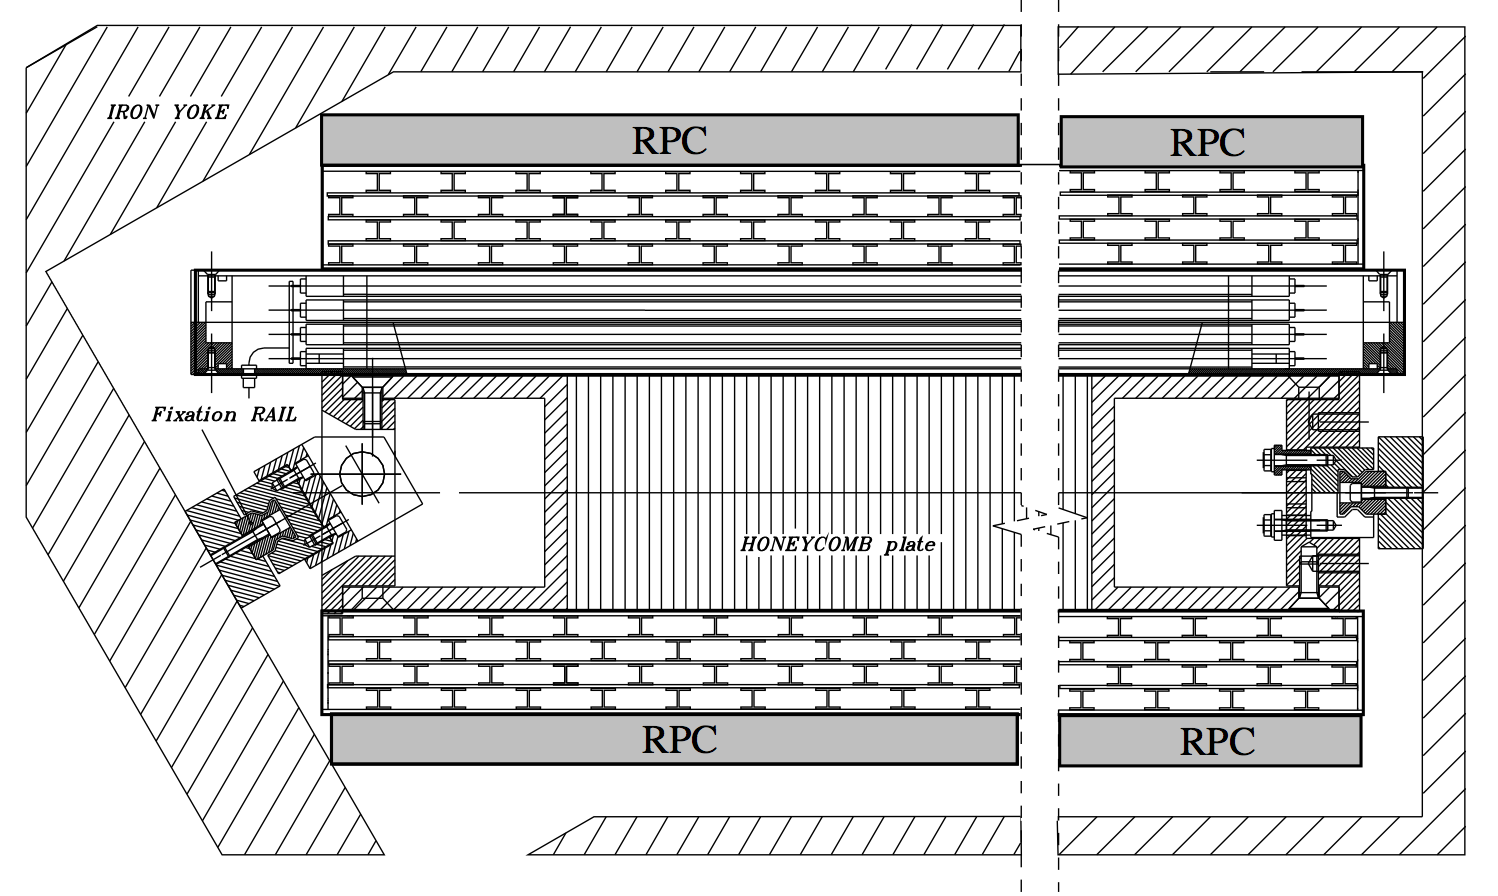
\includegraphics[angle=-0,width=0.8\textwidth]{2_LHC_and_CMS/pics/cms_dt.png}
\caption{Cross-section view of a DT module.
\label{fig:dt_module}
}
\end{center}
\end{figure}


Each SL is made of four stacked layers of tubes staggered by half a cell. This configurations eliminates blind spots and allow for an easy measurement of the muon crossing time by averaging the drift times. Each tube has a rectangular cross-section of $13\times42$ mm\sq ~and is filled with a gas mixture of 85\% Ar and 25\% CO$_2$, leading to a maximum drift time of 380 ns. Each SL has a spatial resolution of about 200 \u m and a time jitter below 5 ns.

\subsubsection*{Cathode Strip Chambers}

The front wheels of the solenoid return yoke are instrumented with multi-wire proportional chambers. Each module has trapezoidal shape and cover either $10\deg$ or $20\deg$ in $\phi$ forming a full disk perpendicular to the beam axis ($r-\phi$ plane). Each of these chambers has the cathode segmented radially in strips (hence the name Cathode Strip Chamber, CSC) of constant $\Delta\phi$ and wires running perpendicular to the strips with spacing of 3.2 mm. 

This design allows to cope with the much higher rate with respect to the barrel and with non uniform and non null magnetic field. 

This detector provides at least three measured point in its acceptance ($1.2 < |\eta| < 2.4$) with a design resolution of approximately 2 mm at trigger level and around 200 \u m after offline reconstruction.

\subsubsection*{Resistive Plate Chambers}

Dual-gap RPC's provide a redundant set of spatial measurements particularly important for trigger purposes, given their response time much shorter than 25~ns. The layout chosen by the CMS collaboration consist of six RPC stations in the barrel and three in the endcaps. RPC stations are placed in proximity (before or after) each CSC or DT station. The first two DT station have two RPC, one before \emph{and} one after, in order to provide at least four position measurements even for low-$p_T$ muons which might not reach the outer stations. Each chamber is operated in avalanche mode and consist of two gaps sharing a segmented pick-up read-out in between, allowing to operate at lower voltages (and therefore lower noise) for the same gain. 

\subsection{Trigger}

As previously said, during the operations LHC delivered an interaction every 50 ns leading to a 20 MHz frequency, half of the design one.
This frequency is well above the storage capabilities of the most modern technologies allowing to accommodate few hundreds of events per second. The inclusive p-p cross-section is hugely dominated by low-$x$ QCD processes that are of no or little interest for this experiment leading to the obvious necessity of a fast-logic to isolate events of some interest for the experiment's physics program while rejecting the others. This event selection of logic, usually referred as \emph{trigger}, is divided in the CMS experiment in two stages: the \emph{level one} (L1) trigger and the \emph{high level trigger} (HLT). 

The L1 trigger decision is based on a coarse reconstruction of the event performed by custom electronics largely mounted directly on the detector. The maximum processing time (called \emph{latency}) is 3.2 \u s. During this time the event is stored on the detector electronics in pipelined memories. Due to timing constraints only inputs from the calorimeters and from the muon system are processed. For the purpose of triggering the calorimeter segmentation is reduced into the so-called \emph{trigger-towers}. Calorimeters provide to the decision logic a set of important physics variables like the missing transverse energy ($E_T^{miss}$), the scalar sum of the transverse hadronic activity ($H_T$), the number of jets above different energy thresholds and the locations of towers compatible with a \emph{minimal ionizing particle} (MIP) and its isolation. Electron and photon identification is also performed looking at the jet hadronic over electromagnetic energy ratio ($H/E$) and cluster shape, performed with the aid of a look-up table. Muon information is mainly provided by DT and CSC subdetectors complemented by the sheer time resolution of RPC for bunch crossing assignment as well as ghost-tracks removal. Muons trajectories are roughly reconstructed by the detector dedicated electronics and then sent to an additional module that merges the information coming from the different stations and subdetectors to assess the transverse momentum  and charge. These informations are complemented by the ones coming from the calorimeters providing isolation values.

The final decision is taken by modules located outside the detector. These modules exploit FPGA's to achieve fast response while allowing for modification of the algorithms to cope with the evolution the instantaneous luminosity or new physics demands. The maximum output frequency for L1 is 1 kHz.

Once the L1 trigger decision is made the full event is read from the detectors buffers and sent to the online \emph{Data Quality Monitoring} (DQM) and to the HLT farm, consisting of over a thousand commercial processors working in parallel. During the HLT decision a simplified version of the CMS offline event reconstruction is performed. Time consuming tasks such as tracking are performed only around the objects that caused the L1 trigger to fire and more complex algorithms like \b-tagging and \t~identification are performed with a simplified version. During this trigger stage decision are taken based on more complex algorithms and a more refined reconstruction allowing to reduce the event rate to roughly 300Hz, which is within the storage and processing capabilities of the CERN facilities. Beeing completely software-based, the HLT is far more flexible and fast evolving than L1 trigger, allowing to cope with the fast changing machine conditions during 2010 and 2011 runs and to achieve a level of refinement beyond the most optimistic forecasts made at the start-up.

Once the event is also accepted by the HLT it is transferred to the CERN computing center for storage and reconstruction.

\section{Data storage and processing}

Events recorded from the detector are stored in \emph{RAW} format, a data format that contains all the digitalized output of the single subdetectors and L1 and HLT information. In order to be useful for physics analysis the trajectory and the nature of the particles originated in the event must be inferred from the hits stored in the RAW event. This process is usually called event reconstruction and is the topic of the following chapter. The CMS detector produces about 15 TB of data for each day of operation.

The reconstruction of collected and simulated data is too CPU and storage demanding to be delegated to a single facility. In order to evenly spread this effort through different computing facilities in various parts of the world, a new computing model was created. The \emph{world wide computing grid} \cite{Malecki:2005gn} allows for fast transfer and de-localized computing throughout the world, allowing to cope with the huge demands that the LHC experiments need to smoothly operate. 

In some sense the grid can be seen as an extension of the batch queue system where the user submit jobs to a single machines, whereas in this case he submits them to clusters of machines, that then take care of submitting those jobs in their peculiar batch queue implementation. Computing facilities are organized in a hierarchical structure called tiers, starting from the facility that receives the data from the detector, called Tier0, scaling to smaller and smaller facilities up to Tier3's providing limited computing and storage for local groups while still being connected to the grid and therefore profiting of the fast transfer abilities. In this system secure access to the resources is ensured by a system of certificates spawning children proxies of limited lifetime.

%displayed
%presented
%illustrated